\subsection{Problema a resolver}

El siguiente ejercicio se da en el contexto de un museo donde se requiere, por cuestiones de seguridad, colocar sensores de forma tal que todo el piso esté cubierto por los lásers que estos emiten. Existen dos tipos de sensores: los direccionales (que emiten señales horizontales o verticales) y los bidireccionales (que emiten señales verticales y horizontales). Los precios de éstos son \$4000 y \$6000 respectivamente. Se pide, también, que un sensor no apunte hacia otro dado que esto podría dejarlos sin funcionar. Además, se pide que ciertos lugares, definidos como \textit{importantes}, sean atravesados por dos lásers simultáneamente. El objetivo del algoritmo a realizar consiste en encontrar una forma de colocar los sensores de manera que el suelo quede completamente cubierto y que los lugares \textit{importantes} estén atravesados por un láser horizontal y otro vertical utilizando el mínimo costo posible. Por otra parte, debe ser tenido en cuenta que el museo cuenta con paredes que pueden interferir los lásers de los sensores.\newline

\newline
\textbf {Formatos de entrada y salida:}\newline
\newline
La entrada del algoritmo contiene una instancia del problema. La primera línea indica las dimensiones $n$ y $m$ de la grilla. A esta línea le siguen $n$ líneas, cada una con $m$ valores separados por espacios, indicando el contenido de cada una de las $n$ x $m$ casillas de la grilla, donde un 0 representa una pared, un 1 representa un casillero libre común y un 2 representa un casillero libre importante.\newline

En el caso en el que el problema no tenga solución, la salida deberá contener únicamente una línea con el valor -1. Caso contrario, la salida debe comenzar con dos números enteros: 
$$S\ C$$ 
donde $S$ es la cantidad de sensores utilizados y $C$ es el costo toal de la solución. Luego, para cada sensor utilizado, debe haber una línea con el siguiente formato: 
$$t\ f\ c$$ 
donde $t$ es el tipode sensor y $(f,c)$ son la fila y columna en donde éste se ubica (la esquina superior izquierda de la grilla es la posición (1,1) y la inferior derecha es la $(n,m)$). Para los sensores cuatridireccionales, $t$ debe valer 1, para los bidireccionales en forma horizontal $t$ debe valer 2 y en forma vertical 3.\newline
\newline
Un ejemplo de este problema es el que está provisto por la cátedra:

\begin{figure}[H]
	\begin{center}
		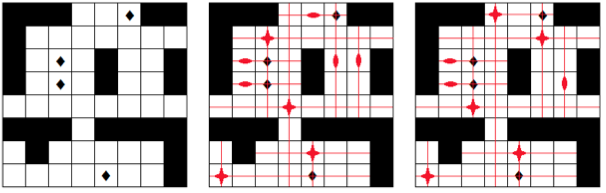
\includegraphics[width=320pt]{../imgs/ej3_ejemploCatedra.png}
	\end{center}
\caption{Un ejemplo y dos soluciones distintas.}
\end{figure}

En el ejemplo de la Figura 1 el museo se ve representado por una cuadricula donde donde los cuadrados blancos representan el suelo, los cuadrados negros representan las paredes y los cuadrados que tienen un rombo dentro representan los lugares importantes, a continuación de la imagen se muestran dos posibles soluciones al problema, en las cuales las cruces rojas representan los sensores bidireccionales, y las lineas rojas gruesas representan los sensores horizontales y verticales, desde estos se extienden lineas rojas que representan el área que cubren estos sensores con lasers.

En el primer caso el costo total es de \$44000 y la segunda solución tiene un costo de \$42000.

\subsection{Resolución coloquial}

Para resolver el problema presentado decidimos utilizar la técnica de $backtracking$. Ésta consiste en evaluar las posibles combinaciones de soluciones del problema almacenándolas hasta llegar a la deseada. Para ello, definimos criterios de parada que nos permitieran decidir si las soluciones parcialmente obtenidas eran candidatas a soluciones válidas.\newline
\newline
Para resolver el problema, representamos el piso entero del museo con una matriz, respetando las paredes y las casillas importantes. Luego, cada elemento de la matriz representa a una baldosa/casillero del piso y almacena el estado de la misma. Esto significa que de acuerdo a si contiene un 0, un 1 o un 2, podemos saber si hay algún sensor en ella o si pasa algún láser por encima.\newline
\newline
Nuestro algoritmo se encarga de recorrer paulatinamente la matriz mencionada y, en cada paso, tomar una decisión sobre el casillero actual para avanzar, luego, al siguiente. Las posibles decisiones son colocar o no algún sensor, empezando por intentar con el sensor bidireccional, para proseguir con el horizontal, luego el vertical y por último ningún sensor. De este modo, se genera un árbol de decisiones cuyas ramas representan un escenario diferente en la distribución de sensores en la matriz que representa nuestra modelo, de esta manera nos garantizamos obtener todas las posibles combinaciones de configuraciones de la matriz. Finalmente, cada casilla tiene que tener un laser pasando por ella excepto pared, las importantes deben tener 2. que ningun sensor le pegue a ningun laser. el costo total de los sensores tiene que ser minimo entre todas las posibles soluciones. me guardo en algun lado la mejor hasta ahora, empezando por la primera (todos bidireccionales) y si esta sol es mejor la reemplazo. tomamos todas estas configuraciones, chequeamos cuales son soluciones correctas y nos quedamos con la que minimiza el costo de los ContarSensores.
Podas reducen la cantidad se soluciones correctas o incorrectas: una vez que encuentro una sol se guarda el costo y cualquier rama cuyo costo actual sea mayor a mi mejor costo -2000 (dif entre sacar bidireccional y poner un direccional) lo descarta. sobre las importantes no puede haber ningun sensor bidireccional. no puede haber ningun sensor vertical en la misma linea que un casillero importante, lo mismo para horizontales en la vertical. si tengo un sensor vertical en una linea no puedo poner ninguno horizontal porque le va a pegar. analogamente de horizontales a vertical.
\newline


\subsection{Demostración de correctitud}

Para demostrar la correctitud de nuestro algoritmo desarrollaremos los siguientes tres items:
\begin{itemize}
\item Nuestro algoritmo genera todas las combinaciones posibles en cada casillero.
\item Las podas utilizadas no alteran el resultado final.
\item La solucion es optima, es decir, no existe otra cuyo costo sea menor.
\end{itemize}

\textbf{Nuestro algoritmo genera todas las combinaciones posibles en cada casillero.} \newline

Esto lo realiza tomando el primer elemento (ignorando el anterior) e intentando ubicar algun sensor, o ninguno, siempre que este no se encuentre contemplado en las podas o que no rompa los casos especificados
 por el enunciado. Como resultado, por cada elemento, puede generar 4 casos posibles: \newline
 $sin$ $sensor$ \newline
 con $sensor$ $bidireccional$ $horizontal$  \newline
 con $sensor$ $bidireccional$ $vertical$  \newline
 con $sensor$ $cuatridireccional$ \newline
  Asi sucesivamente con cada cuadricula, logrando asi, generar todas las permutaciones factibles. 

\textbf{Las podas utilizadas no alteran el resultado final} \newline


\textbf{La solucion es optima, es decir, no existe otra cuyo costo sea menor} \newline


nuestro algoritmo genera todas las combinaciones posibles en cada casillero. - buscamos el costo minimo entonces descartamos una solucion por ya tener una valida. la solucion eliminada puede llegar a ser correcta pero no va a ser la minima.
- al poner un sensor sobre el casillero importante, se quita la posibilidad de poner otro cuyo laser lo atraviese, luego dicha casilla no va a ser atravesada por dos lasers.
- no debe haber ningun laser pegandole al sensor sino se rompe y ademas podria cambiarse por una mejor solucion
- si tengo un sensor horizontal o vertical restrinjo la linea hasta la pared.

Finalmente, sea $C$ el conjunto de configuraciones posibles de la matriz, si en cada paso puedo probar 4 opciones diferentes para cada casillero disponible, y si mi matriz mide $n*m$, entonces por combinatoria tengo $4^{n*m}$ configuraciones finales posibles de la matriz, como nuestro algoritmo hace esencialmente eso (excepto por las podas y criterios de terminación que no representan soluciones validas) podemos decir que este encuentra todas las posibles configuraciones de la matriz.

Como $C$ representa el conjunto de todas las posibles configuraciones del problema (en particular las que son solucion del problema) entonces la solución óptima, si es que existe alguna, está dentro de ese conjunto, y nuestro algoritmo debería encontrarla y devolverla.

si tuviese una solucion correcta, esta estaria en el arbol de decision....

\subsection{Complejidad del algoritmo}

Pseudocódigo:

\begin{algorithm}[H]
	\SetAlgoLined
	\caption{Algoritmo de Backtracking}
	\KwIn{Matriz $grilla$}
	\KwOut{Lista sensores}
	
	Matriz $mejorGrilla$
	Lista $casillasLibres$\\

	\For{Posicion $p \in grilla$}{
		\If{p esta libre}{
			$casillasLibres \leftarrow p$\\
		}
		\If{$p$ es importante}{
			\textbf{RestringirPorImportantes}(p)\\
		}
	}

	sensores := backtrack($grilla$, $casillasLibres$, $mejorGrilla$)\\

	\textbf{devolver} sensores
\end{algorithm}

\begin{algorithm}[H]
	\SetAlgoLined
	\caption{backtrack}
	\KwIn{Matriz $grilla$, Lista $casillasLibres$, Matriz $mejorGrilla$}
	\KwOut{Lista sensores}

    \If{$costoActual$ > $(mejorCostoObtenido - 2000)$}{
        backtrack($grilla$, $casillasLibres$)\\
	}
	
	\If{sensores esta vacio}{
		\If{chequearSolucion($grilla$) \land $ (costoActual $ < $ mejorCostoObtenido)$}{
			$mejorCostoObtenido$ := $costoActual$\\
			$mejorGrilla$ := $grilla$
		}
    }

	Casilla $casillaActual$ := Proxima casilla libre \in casillasLibres\\
	
	\If{$¬$sePuedeColocarUnSensor($casillaActual$)}{
		$mejorCostoObtenido$ := $costoActual$\\
		$mejorGrilla$ := $grilla$
	}
	
	\If{Puedo poner un sensor bidireccional en $casillaActual$}{
		Restringir por láser bidireccional\\
		Saco casillaActual de casillasLibres\\
		backtrack($grilla$, $casillasLibres$)\\
	}
	\If{Puedo poner un sensor vertical en $casillaActual$}{
		Restringir por láser vertical\\
		Restringir casilleros horizontales\\
		Saco casillaActual de casillasLibres\\
		backtrack($grilla$, $casillasLibres$)\\
	}
	\If{Puedo poner un sensor horizontal en $casillaActual$}{
		Restringir por láser horizontal\\
		Restringir casilleros verticales\\
		Saco casillaActual de casillasLibres\\
		backtrack($grilla$, $casillasLibres$)\\
	}

	Dejo el casillero en blanco\\
	backtrack($grilla$, $casillasLibres$)\\

	\textbf{devolver} ContarSensores($grilla$)
\end{algorithm}

\subsection{Código fuente}

\subsection{Complejidad del algoritmo}

Veamos paso a paso la complejidad del algoritmo de backtracking:

En la linea 1 se obtienen las posiciones libres de la grilla, esto se obtiene recorriendo secuencialmente todas las posiciones de la matriz y en cada paso pregunta si es una casilla libre o no, esta pregunta se hace en tiempo constante y recorrer todos los elementos tiene una complejidad de O($n*m$).



\subsection{Instancias posibles}
Para verificar la correctitud de nuestro programa, dispusimos variar estratégicamente las instancias de entrada al ejecutarlo.
\begin{itemize}
\item En primer lugar, ejecutamos el programa ingresando una única casilla libre, siendo ésta un lugar importante. Dicha prueba se realizó con el fin de verificar que nuestro algoritmo devolviera $-1$ dado que no existe la posibilidad de insertar 2 lásers en ese espacio, siendo este el requisito para los espacios importantes.\newline

\textbf{Parámetro de entrada:} 
$$3\ \ 3$$
$$0\ \ 0\ \ 0$$
$$0\ \ 2\ \ 0$$
$$0\ \ 0\ \ 0$$
\textbf{Parámetro de salida:} $$-1$$\newline
\item Por otra parte, probamos el programa para un museo conformado únicamente por paredes, en otras palabras, el caso vacío. Lo relevante de este caso es que nuestro algoritmo lo considera y otorga, como salida, que la solución es no colocar ningún láser.\newline




\textbf{Parámetro de entrada:} 
$$3\ \ 3$$
$$0\ \ 0\ \ 0$$
$$0\ \ 0\ \ 0$$
$$0\ \ 0\ \ 0$$
\textbf{Parámetro de salida:} $$0\ \ 0$$\newline
\item Otro caso interesante es analizar la solución obtenida al tener todos espacios libres. La idea de dicho caso consiste en comprobar que el algoritmo devuelve la solución más económica del problema.\newline

\textbf{Parámetro de entrada:} 
$$3\ \ 3$$
$$1\ \ 1\ \ 1$$
$$1\ \ 1\ \ 1$$
$$1\ \ 1\ \ 1$$
\textbf{Parámetro de salida:} 
$$3\ \ 12000$$
$$2\ \ 0\ \ 0$$
$$2\ \ 1\ \ 2$$
$$2\ \ 2\ \ 0$$
\newline

\item Por otra parte, resulta importante corroborar la solución en el caso en el que todos los espacios son importantes. En este caso particular no existe solución ya que no podrían pasar dos lásers por el mismo casillero especial sin que uno de estos toque a otro láser.\newline

\textbf{Parámetro de entrada:} 
$$3\ \ 3$$
$$2\ \ 2\ \ 2$$
$$2\ \ 2\ \ 2$$
$$2\ \ 2\ \ 2$$
\textbf{Parámetro de salida:} $$-1$$\newline

\item Otra situación posible es en la que se encuentran alternados los casilleros de piso y pared. De este caso puede destacarse que no es posible aplicar ninguna de las podas mencionadas.\newline
\textbf{Parámetro de entrada:} 
$$3\ \ 3$$
$$1\ \ 0\ \ 1$$
$$0\ \ 1\ \ 0$$
$$1\ \ 0\ \ 1$$
\textbf{Parámetro de salida:} 
$$5\ \ 20000$$
$$2\ \ 0\ \ 0$$
$$2\ \ 0\ \ 2$$
$$2\ \ 1\ \ 1$$
$$2\ \ 2\ \ 0$$
$$2\ \ 2\ \ 2$$

\begin{figure}[H] % indico que voy a poner una figura y [h] indica que la posición relativa, tambien puedo usar t = top entre otros.
\hfill
\begin{minipage}[t]{.45\textwidth}
\begin{center}
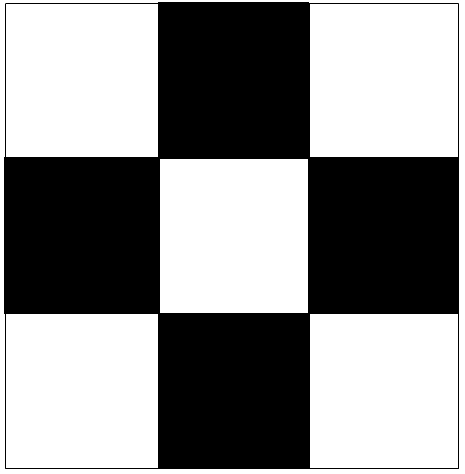
\epsfig{file=instanciaposible_ej3_in5.jpg, scale=0.15} % primera imagen colocada a la izquierda
\caption{Entrada de la instancia posible Nº1.}
\label{fig-tc1}
\end{center}
\end{minipage}
\hfill
\begin{minipage}[t]{.45\textwidth}
\begin{center}
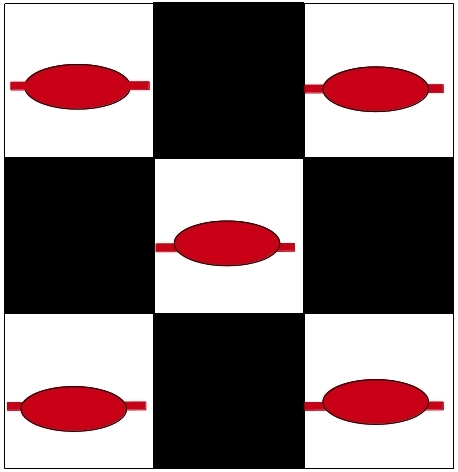
\epsfig{file=instanciaposible_ej3_out5.jpg, scale=0.15} % segunda imagen colocada a la derecha
\caption{Salida de la instancia posible Nº1.}
\label{fig-tc2}
\end{center}
\end{minipage}
\hfill
\end{figure}

\item Por último, se encuentra el caso en el que coexisten los 3 tipos de casilleros, siendo éste el mas típico del problema. \newline

\textbf{Parámetro de entrada:} 
$$3\ \ 3$$
$$1\ \ 1\ \ 1$$
$$1\ \ 2\ \ 0$$
$$0\ \ 0\ \ 1$$
\textbf{Parámetro de salida:} 
$$3\ \ 14000$$
$$1\ \ 0\ \ 1$$
$$2\ \ 1\ \ 0$$
$$2\ \ 2\ \ 2$$
\newline
\end{itemize}

\subsection{Testing}
Para realizar las pruebas de complejidad, generamos instancias aleatorias de pesos de cajas alterando la cantidad de las mismas pero manteniendo estático el peso máximo de carga de los camiones en 120 \unit{kg}. Estas instancias fueron generadas en $C++$ con la función $rand()$ de forma tal a poder acotarlas por la capacidad de carga de los camiones. La cantidad de cajas generadas se comprendió entre 5000 y 100000, agregando de a 5000 en cada iteración. De este modo, logramos medir las pruebas de nuestro algoritmo para comprobar que la complejidad correspondiera con la mencionada anteriormente.

